\documentclass{article}
\usepackage{amsmath}
\usepackage{amssymb}
\setlength{\parindent}{0pt}

\usepackage{tikz}

\usepackage{graphicx}
\usepackage[a4paper, left=1.5in, right=1.5in, top=1.5in, bottom=1.5in]{geometry}
\usepackage{xcolor}

\usepackage{pgfplots}
\usetikzlibrary{intersections,angles,quotes}
\usepgfplotslibrary{fillbetween}

\title{Calculus 101}

\author{alexander}
\date{\today}

\begin{document}
\maketitle

\section*{Introduction}

Calculus is the study of rates of change and the accumulation of quantities.\\

the least common multiple of two (or more) numbers is the smallest number that is a multiple of both (or all) of them:
	\begin{itemize}
		\item multiples of 4: 4, 8, \textcolor{red}{12}, 16, 20
		\item multiples of 6: 6, \textcolor{red}{12}, 18, 24
	\end{itemize}

the greatest common factor of two (or more) numbers is the largest number that divides both (or all) of them without a remainder:
	\begin{itemize}
		\item factors of 12: 1, 2, 3, 4, \textcolor{red}{6}, 12
		\item factors of 18: 1, 2, 3, \textcolor{red}{6}, 9, 18
	\end{itemize}

\textbf{inequalities and absolute value:}
	\begin{itemize}	
		\item $[a, b] = a \leq x \leq b$
		\item $(a, b) = a < x < b$
		\item $[a, b) = a \leq x < b$
		\item $(a, b] = a < x \leq b$
		\item $(-r, r) = \lvert x\rvert < r$
		\item $(c - a, c + a) = \lvert x - c\rvert < a = c - a < x < c + a$
	\end{itemize}

\textbf{triangle inequality}\\

$\lvert a + b\rvert \leq \lvert a \rvert + \lvert b\rvert \to (\lvert a + b\rvert)^2 \leq (\lvert a \rvert + \lvert b\rvert)^2$\\

if you square any real number you will get a non-negative result ($(x)^2 = (-x)^2$)
	\begin{enumerate}
		\item $(a + b)^2 \leq (\lvert a\rvert + \lvert b\rvert)^2$
		\item $a^2 + 2ab + b^2 \leq (\lvert a\rvert)^2 + 2\lvert a\rvert\lvert b\rvert + (b)^2$
		\item $2ab \leq 2\lvert a\rvert\lvert b \rvert$
		\item $ab \leq \lvert a\rvert\lvert b\rvert$
	\end{enumerate}

\textbf{lines equations:}\\
	\begin{itemize}
		\item $(\frac{x_1 + x_2}{2}, \frac{y_1 + y_2}{2})$
		\item $\frac{y_2 - y_1}{x_2 - x_1}$
		\item $y = mx + b$
		\item $y - y_1 = m(x - x_1)$
		\item $Ax + By = C$ 
	\end{itemize}

\textbf{eqautions forms:}
	\begin{itemize}
		\item conic sections and lines: $Ax^2 + Bxy + Cy^2 + Dx + Ey + F = 0$
			\begin{itemize}
				\item lines
				\item parabolas
				\item circles
				\item ellipses
				\item hyperbolas
			\end{itemize}
		\item parametric form: $\begin{cases} x = f(t) \\ y = g(t) \end{cases} \quad \text{for } t \in [a, b]$ 
		\item polar form: $r = f(\theta)$
		\item matrix form:

			\begin{itemize}
				\item $\begin{cases} a_{11} x_1 + a_{12} x_2 + \cdots + a_{1n} x_n = b_1 \\ a_{21} x_1 + a_{22} x_2 + \cdots + a_{2n} x_n = b_2 \\ \vdots \\ a_{m1} x_1 + a_{m2} x_2 + \cdots + a_{mn} x_n = b_m \end{cases}$ 
				\item $ \underbrace{\begin{bmatrix} a_{11} & a_{12} & \cdots & a_{1n} \\ a_{21} & a_{22} & \cdots & a_{2n} \\ \vdots & \vdots & \ddots & \vdots \\ a_{m1} & a_{m2} & \cdots & a_{mn}\end{bmatrix} }_{A} \cdot \underbrace{ \begin{bmatrix} x_1 \\ x_2 \\ \vdots \\ x_n \end{bmatrix} }_{\mathbf{x}} = \underbrace{ \begin{bmatrix} b_1 \\ b_2 \\ \vdots \\ b_m \end{bmatrix} }_{\mathbf{b}}$
			\end{itemize}
	\end{itemize}

\textbf{distance:}	
	\begin{itemize}
		\item $\sqrt{(x_2 - x_1)^2 + (y_2 - y_1)^2}$
	\end{itemize}	

\textbf{pythagorean:}
	\begin{itemize}
		\item $a^2 = b^2 + c^2$
	\end{itemize}

\textbf{triangle:}
	\begin{itemize}
		\item $A = \frac{1}{2}bh$
		\item $A = \frac{1}{2}ab\sin(\theta)$
	\end{itemize}

\textbf{circle:}	
	\begin{itemize}	
		\item $C = 2\pi r$
		\item $A = \pi r^2$ 
	\end{itemize}

\textbf{sector of circle:}
	\begin{itemize}
		\item $A = \frac{1}{2}r^2\theta$
		\item $S = r\theta$
	\end{itemize}

\textbf{sphere:}
	\begin{itemize}
		\item $V = \frac{4}{3}\pi r^3$
		\item $A_s = 4\pi r^2$
	\end{itemize}

\textbf{cylinder:}
	\begin{itemize}
		\item $V = \pi r^2h$
	\end{itemize}

\textbf{cone:}
	\begin{itemize}
		\item $V = \frac{1}{3}\pi r^2h$
		\item $A_s = \pi r\sqrt{r^2+h^2}$
	\end{itemize}

\textbf{cone with arbitrary base: where A is the area of the base:}
	\begin{itemize}
		\item $V = \frac{1}{3}Ah$
	\end{itemize}

\textbf{exponents and logs:} 
	\begin{itemize}
		\item $x^mx^n = x^{m+n}$
		\item $\frac{x^m}{x^n} = x^{m-n}$
		\item $(x^m)^n = x^{mn}$
		\item $x^{-n} = \frac{1}{x^n}$
		\item $(xy)^n = x^ny^n$
		\item $(\frac{x}{y})^n = \frac{x^n}{y^n}$ \item $x^{1/n} = \sqrt[n]{x}$
		\item $x^{\frac{m}{n}} = \sqrt[n]{x^m} = (\sqrt[n]{x})^m$
		\item $\log_ax = y \leftrightarrow a^y = x$
		\item $\log_a(xy) = \log_ax + \log_ay$
		\item $\log_a(a^x) = x$
		\item $a^{\log_a x} = x$
		\item $\log_a(\frac{x}{y}) = \log_ax - \log_ay$
		\item $\log_a1 = 0$
		\item $\log_aa = 1$
		\item $\log_a(x^r) = r\log_ax$
		\item $\log_ba = \frac{\log_ca}{\log_cb}$
	\end{itemize}

\textbf{factoring:}
	\begin{enumerate}
		\item $x^2 - 5x + 6$
		\item $(x - 3)(x - 2)$
	\end{enumerate}

\textbf{factoring by grouping:}
	\begin{enumerate}
		\item $3x^2 -8x + 4$
		\item $3x^2 - 6x -2x + 4$
		\item $(3x^2 - 6x) + (-2x + 4)$
		\item $3x(x - 2) - 2(x - 2)$
		\item $(3x - 2)(x-2)$
	\end{enumerate}

\textbf{completing the square:}
	\begin{enumerate}
		\item $3x^2 + 7x + 4$
		\item $3(x^2 + \frac{7}{3}x + 4)$
		\item $3((x^2 + \frac{7}{3}x) + 4)$
		\item $3((x^2 + \frac{7}{3} + \frac{49}{36}) - \frac{49}{36}) + 4$
		\item $3((x + \frac{7}{6})^2 - \frac{49}{36}) + 4$
		\item $3(x + \frac{7}{6})^2 - \frac{49}{12} + 4$
		\item $4(x + \frac{7}{6})^2 - \frac{49}{12} + 4$
		\item $3(x + \frac{7}{6})^2 - \frac{1}{12}$
	\end{enumerate}

\textbf{obtaining solutions:}
	\begin{enumerate}
		\item $ax^2 + bx + c = 0$
		\item $a(x - h)^2 + k = 0$
		\item $a(x - h)^2 = k'$ (if you find that k prime is negative you will have complex solutions) 
		\item $(x - h)^2 = \frac{k'}{a}$ 
		\item $x - h = \pm \sqrt{\frac{k'}{a}}$
		\item $x = \pm \sqrt{\frac{k'}{a}} + h$
	\end{enumerate}

\textbf{derivation of completing the square:}
	\begin{enumerate}
		\item $ax^2 + bx + c = 0$
		\item $x^2 + \frac{b}{a}x + \frac{c}{a} = 0$
		\item $x^2 + \frac{b}{a}x + (\frac{b}{2a})^2 - (\frac{b}{2a})^2 + \frac{c}{a} = 0$
		\item $(x + \frac{b}{2a})^2 = (\frac{b}{2a})^2 - \frac{c}{a}$
	
		\item $(x + \frac{b}{2a})^2 = (\frac{b^2}{4a^2}) - \frac{4ac}{4a^2}$
		\item $(x + \frac{b}{2a})^2 = \frac{b^2 - 4ac}{4a^2}$
		\item $x + \frac{b}{2a} = \pm \frac{\sqrt{b^2 - 4ac}}{2a}$
		\item $x = -b \pm \frac{\sqrt{b^2 - 4ac}}{2a}$
	\end{enumerate}

\textbf{rational root theorem:}\\

If a polynomial with integer coefficients has any rational roots, then those roots must be of the form: $\frac{p}{q}$ where $p$ is a factor of the constant term and $q$ is a factor of the leading term coefficient.\\

consider $f(x) = x^3 - 6x^2 + 11x - 6$\\
so, the possible values for $p$: $\pm1$, $\pm2$, $\pm3$, $\pm6$ and the possible values for $q$: $\pm1$\\
now form all possible $\frac{p}{q}$: $\pm\frac{1}{1}$, $\pm\frac{2}{1}$, $\pm\frac{3}{1}$, $\pm\frac{6}{1}$\\
You can test each value by plugging into the polynomial to see if it equals 0. If it does, it is a root, and you can factor out that term. Keep in mind that not all polynomials have rational roots. Some roots may be irrational (like $\sqrt{2}$) or complex (involving $i$)\\

$f(1) = 1^3 - 6(1)^2 + 11(1) - 6 = 0$ so now we now that $(x - 1)$ is a factor\\
we can now reduce the polynomial $\frac{x^3 - 6x^2 + 11x - 6}{(x - 1)}$ and now we know that $x^3 - 6x^2 + 11x - 6 = (x - 1)(x^2 - 5x + 6)$ as you can see the solutions are $(x - 1)(x - 2)(x - 3)$\\


\textbf{complex numbers $\sqrt{-1} = i$}\\

a complex number is made up of a real part ($a$) and an imaginary part ($b$) like so: $z = a + bi$ a complex conjugate would be written as so: $\overline{z} = a - bi$...notice that $z + \overline{z} = 2Re(z)$ you can use the complex conguate to help in divition problems with complex numbers like so:
	\begin{enumerate}
		\item $\frac{1 + 2i}{4 - 5i}$
		\item $\frac{1 + 2i}{4 - 5i}\frac{4 + 5i}{4 + 5i}$
		\item $\frac{4 + 5i + 8i - 10}{16 - 20i + 20i - 25i^2}$
		\item $\frac{-6 + 13i}{41}$
		\item $\frac{-6}{41} + \frac{13i}{41}$	
	\end{enumerate}

note that multiplying a complex number by its complex conjugate will give you a real number: $z \cdot \overline{z} = (a + bi)(a - bi) = (a^2) - (bi^2) = a^2 + b^2 = (\lvert z \rvert)^2$\\

difference of squares:
	\begin{itemize}
		\item $x^2 - y^2$
		\item $(x + y)(x - y)$
		\item $x^2 + xy -xy - y^2$
	\end{itemize}

sum of squares:
	\begin{enumerate}
		\item $x^2 + y^2 = x^2 - (-1y^2)$
		\item $x^2 - i^2y^2 = x^2 - (iy)^2$
		\item $(x + iy)(x - iy)$
	\end{enumerate}

example:
	\begin{enumerate}
		\item $36a^8 + 2b^6$
		\item $(6a^4)^2 + (\sqrt{2}b^3)^2$
		\item $(6a^4)^2 - (-1)(\sqrt{2}b^3)^2$
		\item $(6a^4)^2 - (i\sqrt{2}b^3)^2$
		\item $(6a^4 + i\sqrt{2}b^3)(6a^4 - i\sqrt{2}b^3)$
	\end{enumerate}

rectangular form: $z = a + bi$\\
	\begin{itemize}
		\item $\cos(\theta) = \frac{a}{r}$ and $\sin(\theta) = \frac{b}{r}$
		\item $r\cos(\theta) = a$ and $r\sin(\theta) = b$
	\end{itemize}
polar form: $z = r(\cos(\theta) + i\sin(\theta))$
	\begin{itemize}
		\item $r = \overline{z} = \sqrt{a^2 + b^2}$
		\item $\theta = \tan^{-1}(\frac{b}{a})$
	\end{itemize}
eulers form: $re^{i\theta}$\\

given $z = -1 + i\sqrt{3}$ find $z^4$ in both polar and rectangular form
	\begin{enumerate}
		\item $\lvert z\rvert = \sqrt((-1)^2 + (\sqrt(3)^2)) = \sqrt{1 + 3} = 2$ (notice how here we take the principal square root because magnitude (distance) has no direction)
		\item $\theta = \tan^{-1}(\frac{\frac{\sqrt{3}}{2}}{\frac{-1}{2}}) = -60^{\circ}$ (calculator will give you angles between $\frac{-\pi}{2}$ and $\frac{\pi}{2}$ because that is the period of arctan)
		\item the vector is in Q2 so $-60^{\circ} + 180^{\circ} = 120^{\circ}$
		\item $z = 2(\cos(120^{\circ}) + i\sin(120^{\circ}))$
		\item $z^2 = 4(\cos(240^{\circ}) + i\sin(240^{\circ}))$		
		\item $z^3 = 8(\cos(360^{\circ}) + i\sin(350^{\circ}))$
		\item $z^4 = 16(\cos(120^{\circ}) + i\sin(120^{\circ}))$
		\item $z^4 = 16(\frac{-1}{2}) + 16(\frac{\sqrt{3}}{2})i = -8 + 8\sqrt{3}i$
	\end{enumerate}

so there are three cube roots of one in the complex plane:\\
	\begin{itemize}
		\item $x^3 = 1 \to x^3 - 1 = 0$ 
		\item $1 = 1 + 0i \to 1 = 1e^{2\pi ni}$
		\item $x^3 = 1 \to x^3 = e^{2\pi ni}$
		\item $x = 1^{\frac{1}{3}} \to x = e^{\frac{2\pi n}{3}i}$
	\end{itemize}

\textbf{fundamental theorem of algebra:}\\

Every non-zero polynomial equation ($f(x) \neq 0$) of degree $n$ has exactly $n$ complex roots including multiplicities.\\

$p(x) = ax^n = bx^{n-1} + \ldots + k$ (n complex roots)\\

\textbf{conic sections:}\\

Conic sections come from taking a three dimensional right circular double-napped cone and slicing it with a two dimensional plane. Right means the axis is perpendicular to the base. Circular means the base is a circle. Double-napped means the cone actually consists of two identical cones joined vertex to vertex.\\

A circle is the set of all points in a plane that are equidistant (radius) from a fixed point (center). $d = \sqrt{(x_2 - x_1)^2 + (y_2 - y_1)^2} \to r = \sqrt{(x - h)^2 + (y - k)^2} \to (x - h)^2 + (y - k)^2 = r^2$\\

$x^2 + 4x + y^2 - 6y = 23$:
	\begin{enumerate}
		\item $x^2 + 4x + y^2 - 6y = 23$  
		\item $x^2 + 4x + \frac{16}{4} - \frac{16}{4} + y^2 - 6y + \frac{36}{4} - \frac{36}{4} = 23$ 
		\item $(x + 2)^2 - 4 + (y - 3)^2 - 9 = 23$
		\item $(x + 2)^2 + (y - 3)^2 = 36$
	\end{enumerate}

An ellipse is the set of all point surrounding two foci such that $r_1 + r_2 = \text{constant}$. The midpoint of the line segment connecting the two foci is the center. Ellipses have a major and minor axis of symmetry. At each end of the major axis we can find verticies.\\

$\frac{(x - h)^2}{a^2} + \frac{(y - k)^2}{b^2} = 1$ (vertices: ($h \pm a, k$))\\
$\frac{(x - h)^2}{b^2} + \frac{(y - k)^2}{a^2} = 1$ (vertices: ($h, k \pm a$))\\

The major and minor axis has a length of 2a and 2b repectively. The distance from the center to the vertices are a, and the distance from the center to the covertices are b. The distance from the center to either foci is $a^2 = b^2 + c^2 \to c^2 = a^2 - b^2$ 

A parabola are the set of all point that are equidistant from a fixed point (the focus) and a fixed line (the directrix).\\

$f(x) = -x^2 - 2x + 1$:
	\begin{enumerate}
		\item $-(x^2 + 2x - 1)$
		\item $-(x^2 + 2x + \frac{4}{4} - \frac{4}{4} - 1)$ 
		\item $-((x + \frac{2}{2})^2 - 2)$ 
		\item $-(x + 1)^2 + 2$
	\end{enumerate}

The definition of a hyperbola is similar to that of an ellipse, where there are two foci. While every point on a ellipse has distances to these foci that give a constant sum. Every point on a hyperbola has distances to these foci that give a constant differense. The foci sit on the outside of the branches with the two vertices between them. In between those vertices we have the center which sits on the transverse axis connecting the vertices. The a, b, and c terms from the ellipse will pretty much mean the same things. a is the distance from the center to the vertex. c is the distance from the center to a focus. b is the distance from the center to the co-vertex. The co-vertex does not lie on the hyperbola like it does for an ellipse. However, b helps define the asymptotes, which guide the shape of the branches of the hyperbola. If you form a rectangle centered at $(h, k)$ with dimensions: $\text{width} = 2a$ and $\text{height} = 2b$. The asymptotes pass through the diagonals of this rectangle.

$\frac{(x - h)^2}{a^2} - \frac{(y - k)^2}{b^2} = 1$ (asymptotes: $y = \frac{b}{a}x$ and $y = -\frac{b}{a}x$)\\ 
  
$\frac{(y - k)^2}{a^2} - \frac{(x - h)^2}{b^2} = 1$ (asymptotes: $y = \frac{a}{b}x$ and $y = -\frac{a}{b}x$)\\ 

\textbf{basic classes of functions:}
	\begin{itemize}
		\item polynomials: a sum of terms, where each term is made up of coefficient (a constant multiple) of a power function with a whole number exponent
		\item rational functions: a quotient of two polynomials
			\begin{itemize}
				\item vertical asymptotes: vertical lines $x = a$ where the function grows without bound - usually where the denominator is zero and the numerator is not zero
				\item removable discontinuity: points where the function is not defined due to a factor that cancels out from both the numerator and denominator
				\item hotizontal asymptotes: horizontal lines $y = L$ where the function approaches as $x \to \infty$\\
					\begin{itemize}
						\item deg $\text{P} < \text{deg Q}$ ($y = 0$)
						\item deg $\text{P} = \text{deg Q}$ ($y = \frac{\text{leading coefficient of P}}{\text{leading coefficient of Q}}$) 
						\item deg $\text{P} > \text{deq Q}$ (no horizontal asymptote look for slant instead)
					\end{itemize}
				\item slant asymptote: lines $y = mx + b$ that the function approaces as $x \to \infty$, when the numerator's degree is exactly one more than the denominator's degree...to find them perform polynomial long division and the quotient is the slant asymptotoe
			\end{itemize}
		\item algebraic functions: produced by taking sums, products and quotients of roots or polynomials and rational functions
		\item exponential functions: $f(x) = b^x$ where $b > 0$...the inverse of which is $f(x) = log_bx$
		\item trigonometric functions: built from $\sin(x)$ and $\cos(x)$ are called trigonometric functions.
	\end{itemize}

\textbf{constructing new functions:}\\
If $f$ and $g$ are functions, we may construct new functions by forming the sum, difference, product, and quotient functions: $(f + g)(x) = f(x) + g(x)$, $(f - g)(x) = f(x) - g(x)$, $(fg)(x) = f(x)g(x)$, $(\frac{f}{g})(x) = \frac{f(x)}{g(x)}$. We can also multiply functions by constants. We call this a linear combination: $c_1f(x) + c_2g(x)$. Composition is another important way of constructing new functions. The composition of $f$ and $g$ is the function $f \circ g$ defined by $(f \circ g)(x) = f(g(x))$.\\

\textbf{invertable functions:}\\
A function $f$ is invertible if there exists another function $f^{-1}(x)$ such that: $f^{-1}(f(x)) = x$ and $f(f^{-1}(x)) = x$. This "inverse function" switches input and outputs - it reverses the effect of the original function.\\

A function is invertible if it is one-to-one (horizontal line test). So, this means that different input always produce different outputs.\\

\textbf{special factorizations}
	\begin{itemize}
		\item $x^2 - y^2 = (x + y)(x - y)$
		\item $x^3 + y^3 = (x + y)(x^2 - xy + y^2)$
		\item $x^3 - y^3 = (x - y)(x^2 + xy + y^2)$
	\end{itemize}

\textbf{binomial}
	\begin{itemize}
		\item $(x + y)^2 = x^2 + 2xy + y^2$
		\item $(x - y)^2 = x^2 - 2xy + y^2$
		\item $(x + y)^3 = x^3 + 3x^2y + 3xy^2 + y^3$
		\item $(x - y)^3 = x^3 - 3x^2y + 3xy^2 - y^3$
		\item $(x + y)^n = \sum_{k = 0}^{n} = \binom{n}{k}x^{(n-k)}y^{k}$  
	\end{itemize}

\textbf{scalars, vectors, and matrices}\\

scalar multiplication:\\
$\vec{w} = (1 , 2)$\\
$3\vec{w} = (3, 6)$\\

component form: $\vec{v} = (x, y)$\\
polar form: $\vec{v} = (r\cos(\theta), r\sin(\theta)) = r(\cos(\theta), \sin(\theta))$\\

When you graphically add two vectors you add them tail to head. Vector addition is commutative ($\vec{a} + \vec{b} = \vec{b} + \vec{a}$). Preforming both of these additions graphically will form a parallelogram and the vector that bisects this parallelogram is the solution.\\ 

A system of equations is a set of two or more equations that share the same variables. The goal is to find values for those variable that make all the equations in the system true at the same time. For example, in a system with two equations and two variables (like $x$ and $y$), you are looking for a point $(x, y)$ that satisfies both equations.\\

To solve a system of equations using substitution, you start by solving one of the equations for one variable in terms of the other. Then, you substitute that expression into one of the other equations. This gives you an equation with just one variable (assuming you started with two), which you can solve. Once you find that value, you plug it back into one of the original equations to find the second variable.\\

With elimination, the goal is to eliminate one variable by adding or subtracting the equations. You may need to multiply one or both equations first to make the coefficients of a variable match. Once a variable is eliminated, you solve the resulting equation for the remaining variable, then substitute that value back into one of the original equations to find the other variable.\\

You can only add or subtract matrices if they have the same number of rows and the same number of columns. This is because matrix addition and subtraction is an element-wise operation.\\

$
\begin{bmatrix}
	1 & 2 & 3\\
	4 & 5 & 6
\end{bmatrix}
+
\begin{bmatrix}
	7 & 8 & 9\\
	0 & 1 & 2
\end{bmatrix}
=
\begin{bmatrix}
	8 & 10 & 12\\
	4 & 6 & 6
\end{bmatrix}
$\\\\

$A = 
\begin{bmatrix}
	-2 & 5 & 6\\
	5 & 2 & 7
\end{bmatrix}
$\\

The dimensions of a matrix give the number of rows and columns of the matrix in that order. Since matrix $A$ has 2 rows and 3 columns, it is called a $2 \times 3$ matrix.\\

A zero matrix is a matrix in which all of the entries are 0.\\

$O_{3 \times 3} = 
\begin{bmatrix}
	0 & 0 & 0\\
	0 & 0 & 0
\end{bmatrix}
$\\

Zero matrices play a similar role in operations with matrices as the number zero plays in operations with real numbers. When we add an $m \times n$ zero matrix to any $m \times n$ matrix $A$, we get matrix $A$ back. In other words, $A + O = A$ and $O + A = A$.\\

$
\begin{bmatrix}
	4 & 1\\
	-6 & 2
\end{bmatrix}
+
\begin{bmatrix}
	-4 & -1\\
	6 & -2
\end{bmatrix}
=
\begin{bmatrix}
	0 & 0\\
	0 & 0
\end{bmatrix}
$\\

When we add any $m \times n$ matrix to its opposite, we get the $m \times n$ zero matrix. $A + (-A) = O$ and $-A + A = O$ It is also true that $A - A = O$. This is because subtracting a matrix is like adding its opposite.\\

matrix addition properties (A, B, and C are equal dimensions):
	\begin{itemize}
		\item commutative property of addition: $A + B = B + A$
		\item associative property of addition: $A + (B + C) = (A + B) + C$
		\item additive identity: For any matrix $A$, there is a unique matrix $O$ such that $A + O = A$
		\item additive inverse property: For each $A$, there is a unique matrix $-A$ such that $A + (-A) = O$
		\item closure property of addition: $A + B$ is a matrix of the same dimensions $A$ and $B$
	\end{itemize}

matrix scalar multiplication properties (A and B are matrices of equal dimensions, c and d are scalars, and O is a zero matrix):
	\begin{itemize}
		\item associative property of multiplication: $(cd)A = c(dA)$
		\item distributive properties: $c(A + B) = cA + cB$
		\item multiplicative identity property: $1A = A$
		\item multiplicative properties of zero: $0 \cdot A = O$ and $c \cdot O = O$
		\item closure property of multiplication: $cA$ is a matrix of the same dimensions as $A$
	\end{itemize}

Matrices can be thought of as transformations of the plane, meaning they take points (or vectors) in a 2D space and move or change them in specific ways. Imagine every point in the plane as a vector $
\begin{bmatrix}
x\\
y
\end{bmatrix}
$. When you multiply that vector by a $2 \times 2$ matrix, the output is a new vector $
\begin{bmatrix}
x'\\
y'
\end{bmatrix}$ that represents the transformed point.\\

$
M =
\begin{bmatrix}
	m_{11} & m_{12}\\
	m_{21} & m_ {22}
\end{bmatrix}
$
$
V =
\begin{bmatrix}
V_1 \\
V_2
\end{bmatrix}\\
$\\

the new vector would be $M \cdot v = v'$ or you could do $v_{\text{row}}M^T = v'$\\

What kinds of transformations can matrices do?
	\begin{itemize}
		\item scaling: stretching or shrinking the plane along the x- and/or y-axis
		\item rotation: turning all points around the origin by some angle
		\item reflection: flipping points over a line, like the x-axis or y-axis
		\item shearing: slanting the shape, pushing points sideways or vertically
		\item projection: flattening points onto a line or plane
	\end{itemize}

A column vector and a row vector can contain the same numbers, but their orientation matters a lot, especially when it comes to matrix operations like multiplication.\\

$
\begin{pmatrix}
2 & 5 & -1
\end{pmatrix}
$
$
\begin{pmatrix}
4\\
0\\
3
\end{pmatrix}
=
(2)(4) + (5)(0) + (-1)(3) = 8 + 0 - 3 = 5
$

$
\begin{pmatrix}
4\\
0\\
3
\end{pmatrix}
$
$
\begin{pmatrix}
2 & 5 & -1
\end{pmatrix}
=
\begin{pmatrix}
8 & 0 & 6\\
	20 & 0 & 15\\
-4 & 0 & -3
\end{pmatrix}
$\\\\

The determinant of a square matrix is a special number that represents how the matrix transforms space—specifically, it measures how the matrix scales volume (or area in 2D). If the determinant is zero, it means the transformation squashes space into a lower dimension, losing information. A matrix with a zero determinant is called singular, which means it does not have an inverse. This happens when the matrix’s columns (or rows) are linearly dependent, meaning one column can be expressed as a combination of others. In systems of equations, a singular (determinant-zero) matrix implies the system is either dependent—where the equations overlap and there are infinitely many solutions—or inconsistent, where the equations contradict and have no solution. A system is consistent if it has at least one solution, whether unique or infinite. Thus, the determinant and singularity give essential insight into whether a system can be solved uniquely, infinitely, or not at all.\\

If
$ A = 
\begin{bmatrix}
a & b\\
c & d
\end{bmatrix}
$, then $\text{det}(A) = ad - bc$\\

If
$ A = 
\begin{bmatrix}
a & b & c\\
d & e & f\\
g & h & i\\
\end{bmatrix}
$, then $\text{det}(A) = a(ei - fh) - b(di - fg) + c(dh - eg)$\\

What does it mean to compose matrices? It means that you can apply transformations in sequence by multiplying their matrices together.\\

$T = BA$\\
$v' = B(Av) = (BA)v$\\
$f(x) = Ax$\\
$g(x) = Bx$\\
$g(f(x)) = B(Ax) = (BA)x$\\

properties of matrix multiplication (A, B, and C are n x n matrices, I is the n x n identity matrix and O is the n x n zero matrix):
	\begin{itemize}
		\item the commutative property of multiplication \textcolor{red}{does not hold!} $AB \neq BA$
		\item associative property of multiplication: $(AB)C = A(BC)$
		\item distributive properties: $A(B + C) = AB + AC$ and $(B + C)A = BA + CA$
		\item multiplicative identity property $IA = A$ and $AI = A$
		\item multiplicative property of zero: $OA = O$ and $AO = O$
		\item dimension property: the product of an m x n matrix and an n x k matrix is an m x k matrix
	\end{itemize}

Consider a system of equations like so:
$3x - 2y - z = -1$\\
$2x + 5y + 2 = 0$\\
$-4x - y = 8$\\
$\downarrow$\\

$
\begin{bmatrix}
3 & -2 & -1\\
2 & 5 & 1\\
-4 & -1 & 0
\end{bmatrix}
$
$
\begin{bmatrix}
x\\
y\\
z
\end{bmatrix}
$
$
=
\begin{bmatrix}
-1\\
0\\
8
\end{bmatrix}
$\\\\

$\uparrow$ generalized $A_{n \times n}\vec{x}_{n \times 1} = \vec{b}_{n \times 1}$\\

When the coefficient matrix A is not square, you cannot use the inverse to solve the system because only square matrices can have an inverse, and only non-singular square matrices (with $\text{det}(A) \neq 0$) actually do have an inverse. In an underdetermined system (more variables than equations: $m < n$) you will usually have infintely many solutions, or sometimes none. Here you would use substitution, elimination, parametric solutions, or row-reduction (gaussian elimination). In a overdetermined system (more equations than variables: $m > n$) it might be inconsistent (no solution), or sometimes it has a best-fit solution. Here you would use gaussian elimination, least squares method, or pseudoinverses. There are other methods for square matrices like row-reduction or cramer's rule.\\

$f^{-1}(f(x)) = x$\\
$f(f^{-1}(x)) = x$\\

$A =
\begin{bmatrix}
0 & 1\\
-1 & 0
\end{bmatrix}
$

$B =
\begin{bmatrix}
0 & -1\\
1 & 0
\end{bmatrix}
$\\\\

let $A$ represent a $90^{\circ}$ clockwise rotation and $b$ represent a $90^{\circ}$ counter-clockwise rotation of the unit vectors. Visually speaking, thses two rotation matrices are inverses of each other. Multiplying them in either order gives the identity matrix.\\

to find the $\text{det}(A)_{n \times n}$ use cofactor expansion or row reduction (gaussian elemination). you will need to understand minors and cofactors to compute the determinant this way.\\

the adjugate is the transpose of its cofactor matrix $\text{adj}(A) = [C_{ij}]^T$\\

$A^{-1} = \frac{1}{\text{det}(A)} \cdot \text{adj}(A)$\\

gaussian elimination can also be used to find the inverse by augmenting the matrix\\

$[A \mid I] \to [I \mid A^{-1}]$ often faster for large matrices\\

advanced techniques: LU decomposition/row operations\\

\textbf{probability and combinatorics}
consider a standard deck of cards (no jokers)\\
$P(\text{jack}) = \frac{4}{52} = \frac{1}{13}$\\
$P(\text{hearts}) = \frac{13}{52}$\\

now consider a venn diagram for the following:
$P(\text{J} \cup \text{H}) = \frac{4 + 13 - 1}{52}$\\
since the probability of hearts overlaps with the probability of jacks (jack of hearts) youll have to subtract out the double counting...we say that that are not mutually exclusive otherwise you could just add $P(\text{J}) + P(\text{H})$ if they were mutually exclusive\\

addition rule:\\
$P(\text{A} \cup \text{B}) = P(\text{A}) + P(\text{B}) - P(\text{A} \cap \text{B})$\\

now consider mutually exclusive events:\\
$P(\text{A} \cap \text{B}) = 0$\\
$P(\text{A} \cup \text{B}) = P(\text{A}) + P(\text{B})$\\

multiplication rule for independent events:\\
if two events, A and B, are independent (meaning the occurrence of one does not affect the other), then: $P(\text{A} \cap \text{B}) = P(\text{A}) \cdot P(\text{B})$\\

consider a fair coin:\\
$P(\text{back to back heads}) = \frac{1}{2} \cdot \frac{1}{2}$

now consider dependent events say you have a bag with 3 blue and 2 red balls...what is the probability that the first pull is blue and the second is blue\\
$P(\text{1st blue}) \cdot P(\text{2nd blue} \mid \text{1st blue})$\\

$P(\text{A} \cap \text{B}) = P(\text{B}) \cdot P(\text{A} \mid \text{B}) = P(\text{A}) \cdot P(\text{B} \mid \text{A})$\\

permutations (order matters)\\
$P(n, k) = \frac{n!}{(n - k)!}$\\

combinations (order does not matter)\\
$\binom{n}{k} = \frac{n!}{k!(n - k)!}$\\

a probability distribution describes how likely different outcomes are for a random variable
	\begin{itemize}
		\item a random variable is something that can take on different values due to chance (like rolling a die or counting the number of heads in coin flips)
		\item a probability distribution assigns a probability to each possible value that the variable can take
	\end{itemize}

the expected value of a random variable is the long-run average outcome you would expect if you repeated an experiment many times. think of it as the center or balance point of a probability distribution.\\

$E[X] = \sum_{i=1}^{n} x^i \cdot P(x_i)$\\

\textbf{series}\\

A sequence is an ordered list of numbers following some rule or pattern. You can get each term from the previous one by repeated addition (arithmetic sequence) or repeated multiplication (geometric sequence), or some other rule.\\

examples of other rules:
	\begin{itemize}
		\item fibonacci: 
			each term is the sum of the previous two terms: $F_n = F_{n - 1} + F_{n - 2}$\\
			so the sequence starts: $0, 1, 1, 2, 3, 5, 8, 13, \ldots$
		\item quadtratic:\\
			terms might increase by a pattern that fits a quadratic formula, like $n^2$:\\
			$1, 4, 9, 16, 25 \ldots$
		\item alternating:\\
			terms might alternate between positive and negative, like:\\
			$1, -1, 1, -1, 1, -1, \ldots$
		\item recursive:\\
			terms can be defined using more complex rules involoving previous terms
	\end{itemize}

$a, ar, ar^2, ar^3, \ldots, ar^{n-1}$\\
$S_n = a + ar + ar^2 + \ldots + ar^{n-1}$\\

The \textcolor{blue}{first} term is an expression where the variable r is raised to the \textcolor{blue}{zeroth} power, so the \textcolor{blue}{nth} term is an expression that has r raised to the \textcolor{blue}{n-1} power.\\ 

sum of a finite geometric series ($r \neq 1$):
	\begin{enumerate}
		\item $S_n = a + ar + ar^2 + \ldots + ar^{n-1}$ 
		\item $rS_n = ar + ar^2 + ar^3 + \ldots + ar^{n}$   
		\item $S_n - rS_n = (a + ar + ar^2 + \ldots + ar^{n-1}) - (ar + ar^2 + ar^3 + \ldots + ar^{n})$
		\item $S_n - rS_n = a - ar^n$
		\item $S_n(1 - r) = a(1 - r^n)$
		\item $S_n = a\frac{1 - r^n}{1 - r}$ if $r \neq 1$ 
	\end{enumerate}

$\sum_{k = 1}^{n} ar^{k - 1} = \frac{a(1-r^n)}{1 - r}$\\

The binomial theorem gives a formula for expanding powers of a binomial\\

$(a + b)^n = \sum_{k = 0}^{n} = \binom{n}{k}a^{(n-k)}b^{k}$\\

Each term in the expansion represents on way to choose how many a's and how many b's you take from those n factors\\

Pascal's triangle gives you the binomial coeffiecients used in binomial expansion\\

\begin{center}
\begin{tikzpicture}[scale=1.2, every node/.style={circle, draw, minimum size=7mm, inner sep=0pt, font=\small}]

% Row 1
\node (n11) at (0,0) {1};

% Row 2
\node (n21) at (-1,-1) {1};
\node (n22) at (1,-1) {1};

% Row 3
\node (n31) at (-2,-2) {1};
\node (n32) at (0,-2) {2};
\node (n33) at (2,-2) {1};

% Row 4
\node (n41) at (-3,-3) {1};
\node (n42) at (-1,-3) {3};
\node (n43) at (1,-3) {3};
\node (n44) at (3,-3) {1};

% Row 5
\node (n51) at (-4,-4) {1};
\node (n52) at (-2,-4) {4};
\node (n53) at (0,-4) {6};
\node (n54) at (2,-4) {4};
\node (n55) at (4,-4) {1};

\end{tikzpicture}
\end{center}

$(a + b)^4 = 1a^4b^0 + 4a^3b^1 + 6a^2b^2 + 4a^1b^3 + 1a^0b^4$\\

Each number $\binom{n}{k}$ counts the number of ways to chose k b's (and thus n-k a's) from n total factors of (a+b)\\

$a, a + d, a + 2d, \ldots, a + (n - 1)d$\\

sum of a finite arithmetic sequence:
	\begin{enumerate}
		\item $S_n = a + (a + d) + (a + 2d) + \ldots + [a + (n - 1)d]$ 
		\item $S_n = [a + (n - 1)d] + [a + (n - 2)d] + [a + (n - 3)d] + \ldots + a$
		\item $2S_n = n[2a + (n - 1)d]$ 
		\item $S_n = \frac{n}{2}[2a + (n - 1)d]$
	\end{enumerate}

$\sum_{k = 1}^{n}[a + (k - 1)d] = \frac{n}{2}[2a + (n - 1)d]$

\newpage
\section*{Trigonometry}

\begin{center}
\begin{tikzpicture}[scale=1.5]

  % Draw parallel lines
  \draw[thick] (-3,2) -- (3,2);   % Top parallel line
  \draw[thick] (-3,0) -- (3,0);   % Bottom parallel line

  % Draw transversal
  \draw[thick] (-2.5,-0.5) -- (2.5,2.5);

\end{tikzpicture}
\end{center}

angle relationships formed when a transversal intersects parallel lines:
	\begin{itemize}
		\item complementary angles: two angles whose measures add up to $90^{\circ}$
		\item supplementary angles: two angles whose measures add up to $180^{\circ}$
		\item vertical angles: pairs of opposite angles formed when two lines intersect. they are always equal in measure.
		\item corresponding angles: when a transversal crosses two lines, corresponding angles are pairs located on the same side of the transversal and in matching corners (one interior, one exterior). If the lines are parallel, corresponding angles are equal.
		\item alternate interior angles: angles located between the two lines but on opposite sides of the transversal. if the lines are parallel, these angles are equal.
		\item alternate exterior angles: angles located outside the two lines and on opposite sides of the transversal. if the lines are parallel, these angles are equal.
		\item same-side (consecutive) interior angles: angles that lie between the two lines and on the same side of the transversal. if the lines are parallel, these angles are supplementary (add up to $180^{\circ}$)
	\end{itemize}

circle angle theorems:
	\begin{itemize}
		\item inscribed angles subtended by the same arch are equal
		\item an angle insribed in a semi-circle equals $90^{\circ}$
		\item the angle subtendted by an arc at the center is double the angle subtended by the same arc at any point on the circumference
	\end{itemize}


\begin{center}
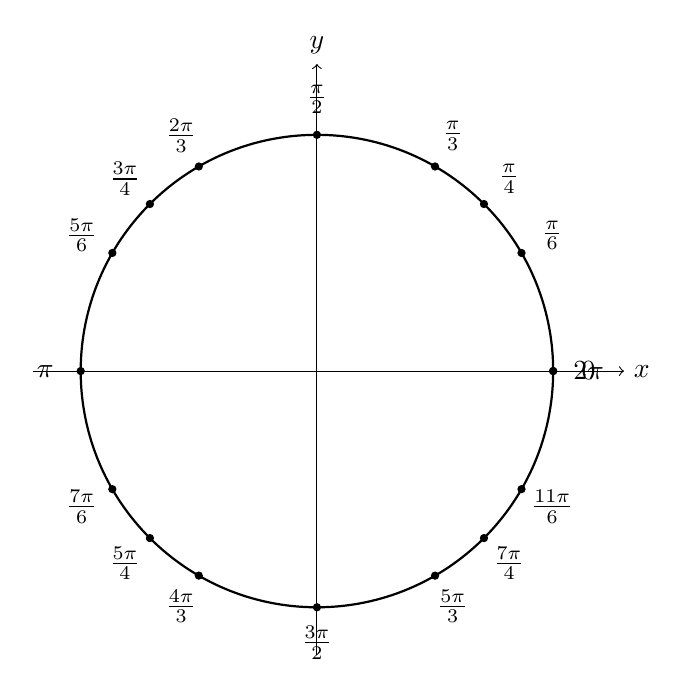
\begin{tikzpicture}[scale=3]
  % Draw the unit circle
  \draw[thick] (0,0) circle(1);

  % Axes
  \draw[->] (-1.2,0) -- (1.3,0) node[right] {\(x\)};
  \draw[->] (0,-1.2) -- (0,1.3) node[above] {\(y\)};

  % Points and angle labels
  \foreach \angle/\label in {
    0/0, 30/\frac{\pi}{6}, 45/\frac{\pi}{4}, 60/\frac{\pi}{3},
    90/\frac{\pi}{2}, 120/\frac{2\pi}{3}, 135/\frac{3\pi}{4},
    150/\frac{5\pi}{6}, 180/\pi, 210/\frac{7\pi}{6},
    225/\frac{5\pi}{4}, 240/\frac{4\pi}{3}, 270/\frac{3\pi}{2},
    300/\frac{5\pi}{3}, 315/\frac{7\pi}{4}, 330/\frac{11\pi}{6},
    360/2\pi}
  {
    \filldraw[black] ({cos(\angle)}, {sin(\angle)}) circle(0.015);
    \node at ({1.15*cos(\angle)}, {1.15*sin(\angle)}) {\(\label\)};
  }
\end{tikzpicture}
\end{center}

$\pi = \frac{\text{circumference}}{\text{diameter}}$\\
$1^\circ = \frac{\pi}{180} \text{radians}$\\

Trigonometric functions are special mathematical functions that originally come from studying right triangles. They relate the size of an angle in a triangle to the ratios of the lengths of the triangle's sides.\\

SOH-CAH-TOA is a mnemonic device that expresses the relationship between the basic trigonometric functions and the ratios of the sides in a right triangle.\\

The triangle definition only works for angles between 0 and $\frac{\pi}{2}$. To extend trig functions to all angles (including negative angles and angles larger then ($2\pi$ or $360^{\circ}$), mathematicians use the unit circle. Thus allowing use to use trig functions on the coordinate plane, enabling graphing and calculus.\\	

\textbf{trigonometric identities:}
\begin{itemize}
	\item $\frac{1}{\cos(\theta)} = \sec(\theta)$	
	\item $\frac{1}{\sin(\theta)} = \csc(\theta) $
	\item $\frac{1}{\tan(\theta)} = \cot(\theta)$
	\item $\sin(\theta + 2\pi) = \sin(\theta)$
	\item $\cos(\theta + 2\pi) = \cos(\theta)$
	\item $\tan(\theta + \pi) = \tan(\theta)$
	\item $\cos(\frac{\pi}{2} - \theta) = \sin(\theta)$
	\item $\sin(\frac{\pi}{2} - \theta) = \cos(\theta)$
	\item $\tan(\frac{\pi}{2} - \theta) = \cot(\theta)$
	\item $\sin(-\theta) = -\sin(\theta)$
	\item $\cos(-\theta) = \cos(\theta)$
	\item $\tan(\theta) = -\tan$
	\item $\sin^2(\theta) + \cos^2(\theta) = 1$
	\item $1 + \tan^2(\theta) = \sec^2(\theta)$
	\item $1 + \cot^2(\theta) = \csc^2(\theta)$
	\item $\cos(A \pm B) = \cos(A)\cos(B) \mp \sin(A)\sin(B)$		
	\item $\sin(A \pm B) = \sin(A)\cos(B) \pm \cos(A)\sin(B)$
	\item $\tan(A \pm B) = \frac{\tan(A) \pm \tan(B)}{1 \mp \tan(A)\tan(B)}$
	\item $\sin(2\theta) = 2\sin(\theta)\cos(\theta)$
	\item $\cos(2\theta) = \cos^2(\theta) - \sin^2(\theta)$		
	\item $\cos(2\theta) = 2\cos^2(\theta) - 1$
	\item $\cos(2\theta) = 1 - 2\sin^2(\theta)$
\end{itemize}

\textbf{law of sines and cosines}\\

	$\frac{\sin(A)}{a} = \frac{\sin(B)}{b} \frac{\sin(C)}{c}$\\
	$a^2 = b^2 + c^2 - 2bc\cos(A)$ (SAS or SSS)

\section*{Limits}

An indeterminate form is a mathematical expression that arises in limits where the limit cannot be directly determined from the form itself because it is ambiguous or undefined in a straightforward way.\\

\textbf{indeterminate forms:}
	\begin{itemize}
		\item $\frac{0}{0}$
		\item $\frac{\infty}{\infty}$
		\item $0 \times \infty$
		\item $\infty - \infty$
		\item $0^0$
		\item $\infty^0$
	\end{itemize}

\textbf{types of discontinuities:}
	\begin{itemize}
		\item removeable: $f(x) = \frac{(x^2 - 1)}{x - 1}$
		\item jump: the left-hand and right-hand limit at the point exist but are not equal
		\item infinite (essential): $f(x) = \frac{1}{x}$
		\item oscillatory: $f(x) = \sin(\frac{1}{x})$
	\end{itemize}

How do the values of a function behave when x approaches a number c, whether or not the function at c is defined?\\
$f(x) = \frac{\sin(x)}{x}$
$f(0) = \frac{\sin(0)}{0} = \frac{0}{0}$\\
Using a calculator you can numerically see that as $x \to 0+$ and $x \to 0-$ the function appears to approach one.\\

\textbf{limit laws} assume that $\lim_{x \to c}f(x)$ and $\lim_{x \to c}g(x)$ exist, then:
	\begin{itemize}
		\item sum law: $\lim{x \to c}(f(x) + g(x)) = \lim_{x \to c}f(x) + \lim_{x \to c}g(x)$
		\item constant multiple law: for any number k, $\lim_{x \to c}kf(x) = k\lim_{x \to c}f(x)$
		\item product law: $\lim_{x \to c}f(x)g(x) = (\lim_{x \to c}f(x))(\lim_{x \to c}g(x)$)
		\item quotient law: if $\lim_{x \to c}g(x) \neq 0$, then $\lim_{x \to c}\frac{f(x)}{g(x)} = \frac{\lim_{x \to c}f(x)}{\lim_{x \to c}g(x)}$
	\end{itemize}

\textbf{continuity at a point:} $\lim{x \to c}f(x) = f(c)$\\

\textbf{laws of continuity} assume that $f(x)$ and $g(x)$ are continuous at a point $x = c$. then the following functions area lso continuous at $x = c$:
	\begin{itemize}
		\item $f(x) + g(x)$ and $f(x) - g(x)$
		\item $kf(x)$ for any constant k
		\item $f(x)g(x)$
		\item $\frac{f(x)}{g(x)}$ if $g(c) \neq 0$
	\end{itemize}

\textbf{continuity of composite functions} let $F(x) = f(g(x))$ be a composite function. If $g$ is continuous at $x = c$ and $f$ is continuous at $x = g(c)$, then $F(x)$ is continuous at $x = c$.\\

\textbf{squeeze theorem} assume that for $x \neq c$ (in some open interval containing $c$), $l(x) \leq f(x) \leq u(x)$ and $\lim_{x \to c}l(x) = \lim_{x \to c}u(x) = L$ then $\lim_{x \to c}f(x)$ exists and $\lim_{x \to c}f(x) = L$\\

\textbf{important trigonometric limits:}
	\begin{itemize}
		\item $\lim_{\theta \to 0}\frac{\sin(\theta)}{\theta}$
		\item $\lim_{\theta \to 0}\frac{1 - \cos(\theta)}{\theta}$
	\end{itemize}

\textbf{intermediate value theorem:} if $f(x)$ is continuous on a closed interval $[a, b]$ and $f(a) \neq f(b)$, then for every value $M$ between $f(a)$ and $f(b)$, there exists at least one value $c \in (a, b)$ such that $f(c) = M$.\\

\textbf{existence of zeros:} if $f(x)$ is continuous on $[a, b]$ and if $f(a)$ and $f(b)$ are nonzero and have opposite signs, then $f(x)$ has a zero in $(a, b)$.\\

we can locate zeroes of functions to arbitrary accuracy using the \textbf{bisection method}.\\
$f(x) = \cos^2(x) - 2\sin(\frac{x}{4})$\\
$f(0) = 1 > 0$, $f(2) \approx -0.786 < 0$\\
we can guarantee that $f(x) = 0$ has a solution in $(0, 2)$. we can locate a zero more accurately by dividing $[0, 2]$ into two intervals $[0, 1]$ and $[1, 2]$. one of these must contain a zero of $f(x)$. to determine which, we evalutate $f(x)$ at the midpoint $m = 1$. a calculator gives $f(1) \approx -0.203 < 0$, and since $f(0) = 1$, we see that $f(x)$ takes opposite signs at the endpoints of $[0, 1]$. therefore, $(0, 1)$ must contain a zero. we discard $[1, 2]$ because both $f(1)$ and $f(2)$ are negative. the bisection method consists of continuing this process until we narrow down the location of the zero to the desired accuracty.\\

\textbf{the size of the gap:}\\
recall that the distance from $f(x)$ to $L$ is $\lvert f(x) - L\rvert$. it is convenient to refer to the quantity $\lvert f(x) - L\rvert$ as the gap between the value $f(x)$ and the limit $L$. lets reexamine the basic trigonometric limit $\lim_{x \to 0}\frac{\sin(x)}{x}$. so 1 tells us that the gap $\lvert f(x) - 1\rvert$ gets arbitrarily small when x is sufficiently close by not equal to 0. suppose we want the gap $\lvert f(x) - 1\rvert$ to be less than 0.2. how close to 0 must x be? $\lvert f(x) - 1\rvert < 0.2$ if $0 < \lvert x\rvert < 1$. if we insist instead that the gap be smaller than 0.004, we can check by zooming in $\lvert f(x) - 1\rvert < 0.004$ if $0 < \lvert x\rvert < 0.15$. it would seem that this process can be continued: by zooming in on the graph, we can find a small interval around $c = 0$ where the gap $\lvert f(x) - 1\rvert$ is smaller than any prescribed positive number. to express this in a precise fasion, we follow time-honored tradition and use the greek letters $\epsilon$ (epsilon) and $\delta$ (delta to denote small numbers specifying the size of the gap and the quantity $\lvert x - c\rvert$, respectively. in our case, $c = 0$ and $\lvert x - c\rvert = \lvert x - 0\rvert = \lvert x\rvert$. The precise meaning is that for every choice of $\epsilon > 0$, there exists some $\delta$ (depending on $\epsilon$) such that $\lvert \frac{\sin(x)}{x} - 1\rvert < \epsilon$ if $0 < \lvert x\rvert < \delta$. the number $\delta$ tells us how close is sufficiently close for a give $\epsilon$.\\

\textbf{formal definition of a limit:}\\
suppose that $f(x)$ is defined for all $x$ in an open interval containing $c$ (but not necessarily at $x = c$). then
\begin{center}$\lim_{x \to c}f(x) = L$\end{center}
if for all $\epsilon > 0$, there exists $\delta > 0$ such that
\begin{center}$\lvert f(x) - L\rvert < \epsilon$ if $0 < \lvert x - c\rvert < \delta$\end{center}

\section*{Differentiation}

\textbf{the derivative} of a function $f$ at $x = a$ is the limit of the difference quotients (if it exists):
\begin{center} $f'(a) = \lim_{h \to 0}\frac{f(a + h) - f(a)}{h}$ \end{center}
when the limit exists, we say that $f$ is differentiable at $x = a$. an equivalent definition of the derivative is
\begin{center} $f'(a) = \lim_{x \to a}\frac{f(x) - f(a)}{x - a}$ \end{center}

\textbf{tangent lines:}\\
assume that $f(x)$ is differentiable at $x = a$. the tangent line to the graph of $y = f(x)$ at $P = (a, f(a))$ is the line through $P$ of slope $f'(a)$. the equation of the tangent line in point-slope form is
\begin{center} $y - f(a) = f'(a)(x - a)$ \end{center}

\textbf{derivative of linear and constant functions:}
	\begin{itemize}
		\item if $f(x) = mx + b$ is a linear function, then $f'(a) = m$ for all $a$
		\item if $f(x) = b$ is a constant function, then $f'(a) = 0$ for all $a$
	\end{itemize}
\newpage

\textcolor{blue}{proof of the power rule}
	\begin{enumerate}
		\item assume that $n$ is a whole number and let $f(x) = x^n$. then $f'(a) = \lim_{x \to a}\frac{x^n - a^n}{x - a}$
		\item to simplify the difference quotient, we need to generalize the following identities: $x^2 - a^2 = (x - a)(x + a)$\\ $x^3 - a^3 = (x - a)(x^2 + xa + a^2)$\\ $x^4 - a^4 = (x - a)(x^3 + x^2a + xa^2 + a^3)$
		\item the generalizaiton is $x^n - a^n = (x - a)(x^{n - 1} + x^{n - 2}a + x^{n - 3}a^2 + \ldots + xa^{n - 2} + a^{n - 1})$
		\item to verify, observe that the right-hand side is equal to\\ $x(x^{n - 1} + x^{n - 2}a + x^{n - 3}a^2 + \ldots + xa^{n - 2} + a^{n - 1})$\\$-a(x^{n - 1} + x^{n - 2}a + x^{n - 3}a^2 + \ldots + xa^{n - 2} + a^{n - 1})$
		\item when we carry out the multiplications, al terms cancle except the first and the last, so $x^n - a^n$ remains, as required. the identity gives us\\ $\frac{x^n - a^n}{x - a} = x^{n - 1} + x^{n - 2}a + x^{n - 3}a^2 + \ldots + xa^{n - 2} + a^{n - 1} (x \neq a)$
		\item therefore,\\ $f'(a) = \lim_{x \to a}(x^{n - 1} + x^{n - 2}a + x^{n - 3}a^2 + \ldots + xa^{n - 2} + a^{n - 1})$\\ $a^{n - 1} + a^{n - 2}a + a^{n - 3}a^2 + \ldots + aa^{n - 2} + a^{n - 1} (\text{n terms})$\\ $na^{n - 1}$
	\end{enumerate}

\textbf{linearity rules} assume that $f$ and $g$ are differentiable functions
	\begin{itemize}
		\item sum rule: the function $f + g$ is differentiable and $(f + h)' = f' + g'$
		\item constant multiple rule: for any constant $c$, $cf$ is differentiable and $(cf)' = cf'$
	\end{itemize}

\textbf{differentiability implies continuity} if $f$ is differentiable at $x = c$, then $f$ is continuous at $x = c$.\\
\textcolor{blue}{Proof:}
	\begin{enumerate}
		\item by definition, if $f$ is differentiable at $x = c$, then the following limit exists: $f'(c) = \lim_{x \to c}\frac{f(x) - f(c)}{x - c}$
		\item our goal is to prove that $f$ is continuous at $x = c$, which means that $\lim_{x \to c}f(x) = f(c)$. To relate the two limits, consider the equation (valid for $x \neq c$) $f(x) - f(c) = (x - c)\frac{f(x) - f(c)}{x - c}$
		\item both factors on the right approach a limit as $x \to c$, so we may apply the limit laws: $\lim_{x \to c}(f(x) - f(c)) = \lim_{x \to c}((x - c)\frac{f(x) - f(c)}{x - c})$
		\item $\lim_{x \to c}(f(x) - f(c)) = (\lim_{x \to c}(x - c)(\lim_{x \to c}\frac{f(x) - f(c)}{x - c})$
		\item $\lim_{x \to c}(f(x) - f(c)) = 0 \cdot f'(c) = 0$
		\item therefore, $\lim_{x \to c}f(x) = \lim_{x \to c}(f(x) - f(c)) + \lim_{x \to c}f(c) = 0 + f(c) = f(c)$, as desired
	\end{enumerate}

\textcolor{blue}{proof of the product rule}
	\begin{enumerate}
		\item we prove the product rule by writing the difference quotient for $f(x)g(x)$ in a vlever way as a sum of two terms. the limit definition of the derivative applied to the product function gives us\\ $(fg)'(x) = \lim_{h \to 0}\frac{f(x + h)g(x + h) - f(x)g(x)}{h}$
		\item the trick is to subtract $f(x + h)g(x)$ and add it back again in the numerator of the difference quotient:\\ $f(x + h)g(x + h) - f(x + h)g(x) + f(x + h)g(x) - f(x)g(x)$
		\item combing terms, we see that the numerator is equal to\\ $f(x + h)(g(x + h) - g(x)) + g(x)(f(x + h) - f(x))$
		\item now write $(fg)'(x)$ as a sum of two limits: \\ $(fg)'(x) = \lim_{h \to 0}f(x + h)\frac{g(x + h) - g(x)}{h} + \lim_{h \to 0}g(x)\frac{f(x + h) - f(x)}{h}$
		\item the use of the sum law is valid, provided that each limit on the right exists. to check that the first limit exist and evaluate it, we note that $f(x)$ is continuous (because it is differentiable) and that $g(x)$ is differentiable:\\ $\lim_{h \to 0}f(x + h)\frac{g(x + h) - g(x)}{h} = \lim_{h \to 0}f(x + h)\lim_{h \to 0}\frac{g(x + h) - g(x)}{h} = f(x)g'(x)$
		\item the second limit is similar:\\ $\lim_{h \to 0}g(x)\frac{f(x + h) - f(x)}{h} = g(x)\lim_{h \to 0}\frac{f(x + h) - f(x)}{g} = g(x)f'(x)$
		\item using the aforementioned we conclude that $fg$ is differentiable and that $(fg)'(x) = f(x)g'(x) + g(x)f'(x)$ as desired.
	\end{enumerate}		

\textcolor{blue}{proof of the quotient rule}
	\begin{enumerate}
		\item start with the definition of the derivative\\ $(\frac{f}{g})'(x) = \lim_{h \to 0}\frac{\frac{f(x + h)}{g(x + h)} - \frac{f(x)}{g(x)}}{h}$
		\item combine the two fractions in the numerator\\ $(\frac{f}{g})'(x) = \lim_{h \to 0} \frac{1}{h} \cdot \frac{f(x + h)g(x) - f(x)g(x + h)}{g(x + h)g(x)}$    
		\item manipulate the numerator\\ $f(x + h)g(x) - f(x)g(x + h) = [f(x + h)g(x) - f(x)g(x)] - [f(x)g(x + h) - f(x)g(x)] = g(x)[f(x + h) - f(x)] - f(x)[g(x + h) - g(x)]$
		\item lets put that back into the limit\\ $(\frac{f}{g})'(x) = \lim_{h \to 0}\frac{g(x)[f(x + h) - f(x)] - f(x)[g(x + h) - g(x)]}{h \cdot g(x + h)g(x)}$ 
		\item split the limit\\ $\lim_{h \to 0}[\frac{g(x)[f(x + h) - f(x)]}{h \cdot g(x + h)g(x)} - \frac{f(x)[g(x + h) - g(x)]}{h \cdot g(x + h)g(x)}]$\\
		\item $(\frac{f}{g})'(x) = \frac{g(x)f'(x) - f(x)g'(x)}{[g(x)]^2}$ 
	\end{enumerate}

\textcolor{blue}{proof of the derivative of sin}
	\begin{enumerate}
		\item $\sin(x + h) = \sin(x)\cos(h) + \cos(x)\sin(h)$
		\item $\sin(x + h) - \sin(x) = \sin(x)\cos(h) + \cos(x)\sin(h) - \sin(x)$ 
		\item $\sin(x + h) - \sin(x) = (\sin(x)\cos(h) - \sin(x)) + \cos(x)\sin(h)$ 
		\item $\sin(x + h) - \sin(x) = \sin(x)(\cos(h) - 1) + \cos(x)\sin(h)$ 
		\item $\lim_{h \to 0}\frac{\sin(x)(\cos(h) - 1)}{h} + \lim_{h \to 0}\frac{\cos(x)\sin(h)}{h}$
		\item $\sin(x)(0) + \cos(x)(1)$
	\end{enumerate}

\textcolor{blue}{proof of the chain rule}
	\begin{enumerate}
		\item $h(x) = f(g(x))$
		\item $h'(x) = \lim_{h \to 0}\frac{f(g(x + h)) - f(g(x))}{h}$
		\item the key idea is to manipulate the difference quotient to introduce $g(x + h) - g(x)$\\ $\frac{f(g(x + h)) = f(g(x))}{h} = \frac{f(g(x + h)) - f(g(x))}{g(x + h) - g(x)} \cdot \frac{g(x + h) - g(x)}{h}$
		\item $h'(x) = \lim_{h \to 0}\frac{f(g(x + h)) - f(g(x))}{g(x + h) - g(x)} \cdot \lim_{h \to 0}\frac{g(x + h) - g(x)}{h}$
		\item this is legitimate only if the denominator $g(x + h - g(x)$ is nonzero. therefore, to continue our proof, we make the extra assumption that $g(x + h) - g(x) \neq 0$ for all $h$ near but not equal to 0. this assumption is not necessary, but without it, the argument is more technical. the second limit on the right is $g'(x)$. the chain rule will follow if we show that the first limit equals $f'(g(x))$. to verify this, set $k = g(x + h) - g(x)$. then $g(x + h) = g(x) + k$ and\\ $\frac{f(g(x + h) - f(g(x)}{g(x + h) - g(x)} = \frac{f(g(x) + k) - f(g(x)}{k}$
		\item since $g(x)$ is differentiable, it is also continuous. therefor $g(x + h)$ tends to $g(x)$ and $k = g(x + h) - g(x)$ tends to zero as $h \to 0$. thus, we may rewrite the limit in terms of $k$ to obtain the desired result:\\ $\lim_{h \to 0}\frac{f(g(x + h)) - f(g(x))}{g(x + h) - g(x)} = \lim_{k \to 0}\frac{f(g(x) + k - f(g(x))}{k} = f'(g(x))$
	\end{enumerate}

\textcolor{blue}{proof of the general power rule}
	\begin{enumerate}
		\item we write $g(x)^n = f(g(x))$, with $f(u) = u^n$. then $f'(u) = nu^{n - 1}$ and, by the chain rule,\\ $\frac{d}{dx}(g(x))^n = f'(g(x))g'(x) = n(g(x))^{n - 1}g'(x)$
	\end{enumerate}

\textbf{shifting and scaling rule} if $f(x)$ is differentiable, then for any constants $k$ and $b$, $\frac{d}{dx}f(kx + b) = kf'(kx + b)$\\

\textbf{implicit differentiation:}\\
to differentiate using the methods covered thus far, we must have a formula for $y$ in terms of $x$, for instance, $y = x^3 + 1$. but suppose that $y$ is determined instead by an equation such as $y^4 + xy = x^3 - x + 2$. in this case, we say that $y$ is defined impplicitly. how can we find the slope of the tangent line at a point on the graph? it may be inconvenient or even impossible to solve for $y$ explicitly as a function of $x$, but we can find $\frac{dy}{dx}$ using the method of implicit differentiation. to illustrate, consider the equation of the unit circle:
	\begin{enumerate}
		\item $x^2 + y^2 = 1$
		\item to compute $\frac{dy}{dx}$, first take the derivative of both sides of the equation and evaluate: \\ $\frac{d}{dx}(x^2 + y^2) = \frac{d}{dx}(1)$
		\item $\frac{d}{dx}(x^2) + \frac{d}{dx}(y^2) = 0$
		\item $2x + \frac{d}{dx}(y^2) = 0$
		\item what should we do with the term $\frac{d}{dx}(y^2)$? we use the chain rule. if we think of $y$ as a function $y = f(x)$, then $y^2 = f(x)^2$, and by the chain rule,\\ $\frac{d}{dx}y^2 = \frac{d}{dx}f(x)^2 = 2f(x)\frac{df}{dx} = 2y\frac{dy}{dx}$
		\item $2x + \frac{d}{dx}(y^2)\to 2x + 2y\frac{dy}{dx}$, and we may solve for $\frac{dy}{dx}$ if $y \neq 0$:
		\item $\frac{dy}{dx} = -\frac{x}{y}$
	\end{enumerate}

\textbf{related rates:}\\
in related rate problems, the goal is to calculate an unknown rate of change in terms of other rates of change that are known. one typical problem involves a ladder learning against a wall. the question is: how fast does the ladder move if the bottom of the ladder is pulled away from the wall at constant speed? what is interesting and perhaps surprising is that the top and bottom travel at different speeds.\\

\textbf{linear approximation:}\\
we can use the derivative to estimate $\Delta f$ without computing it exactly. by definition, the derivative is the limit\\ $f'(a) = \lim_{\Delta x \to 0}\frac{f(a + \Delta x) - f(a)}{\Delta x} = \lim_{\Delta x \to 0}\frac{\Delta f}{\Delta x}$\\ so when $\Delta x$ is small, we have $\frac{\Delta f}{\Delta x} \approx f'(a)$, and thus, $\Delta f \approx f'(a)\Delta x$\\

the linear approximation if often called the tangent line approximation because of the following interpretation. the quantitiy $\Delta f$ is the vertical change from $x = a$ to $a = a + \Delta x$ in the graph of $f(x)$. recall that for a nonvertical straight line, the vertical change is equal to the slope times the horizontal change. since the tangent line has slope $f'(a)$. the vertical change in the tangent line is $f'(a)\Delta x$. what the linear approximation does, therefore, is used the vertical change in the tangent line as an approximation to the vertical change in the graph of $f(x)$. when $\Delta x$ is small, the two quantities are nearly equal.\\

Keep in mind the different roles played by $\Delta f$ and $f'(a)\Delta x$. the quantity of interest is $\Delta f$ and we estimate it by $f'(a)\Delta x$. most importantly, the linear approximation tells us that there is a nearly linear relationship between $\Delta f$ and $\Delta x$ when $\Delta x$ is small.\\

\textbf{linearization:}\\
we can approximate $f(x)$ itself rather than the change $\Delta f$ by rewriting the linear approximation in terms of the variable $x = a + \Delta x$. Then\\ $f(a + \Delta x) - f(a) \approx f'(a)\Delta x$\\ $f(x) - f(a) \approx f'(a)(x - a)$ (since $\Delta x = x - a$)\\ $f(x) \approx f(a) + f'(a)(x - a)$\\ the function on the right, denoted by $L(x)$, is called the linearization of $f(x)$ at $x = a$:\\ $L(x) = f'(a)(x - a) + f(a)$\\ we refer to $x = a$ as the center of the linearization. notice that $y = L(x)$ is the equation of the tangent line to the graph of $f(x)$ at $x = a$\\

\textbf{approximating $f(x)$ by its linearization} assume that $f$ is differentiable at $x = a$ if $x$ is close to $a$, then\\ $f(x) \approx L(x) = f'(a)(x - a) + f(a)$\\

\textbf{extreme values on an interval} let $f(x)$ be a function on an interval I and let $a \in I$. we say that $f(a)$ is the
	\begin{itemize}
		\item absolute minimum of $f(x)$ on $I$ if $f(a) \leq f(x)$ for all $x \in I$
		\item absolute maximum of $f(x)$ on $I$ if $f(a) \geq f(x)$ for all $x \in I$
	\end{itemize}

\textbf{existence of extrema on a closed interval} if $f(x)$ is a continuous function on a closed (bounded) interval $I = [a, b]$, then $f(x)$ takes on a minimum and a maximum value on $I$.\\

\textbf{local extrema} we say that $f(x)$ has a
	\begin{itemize}
		\item at $x = c$ if $f(c)$ is the minimum value of $f$ on some open interval (in the domain of $f$) containing $c$.
		\item at $x = c$ if $f(c)$ is the maximum value of $f(x)$ on some open interval (in the domain of $f$) containing $c$.
	\end{itemize}

\textbf{critical points} a number $c$ in the domain of $f$ is called a critical point if either $f'(c) = 0$ or $f'(c)$ DNE.\\

\textbf{fermat's theorem on local extrema} if $f(c)$ is a local min or max, then $c$ is a critical point of $f$.\\

\textbf{extreme values on a closed interval} assume that $f(x)$ is continuous on $[a, b]$ and let $f(c)$ be the minimum or maximum value on $[a, b]$. then $c$ is either a critical point or one of the endpoints $a$ or $b$.\\

\textbf{rolle's theorem} assume that $f(x)$ is continous on $[a, b]$ and differentiable on $(a, b)$. if $f(a) = f(b)$, then there exists a number $c$ between $a$ and $b$ such that $f'(c) = 0$.\\

\textbf{mean value theorem} assume that $f$ is continuous on the closed interval $[a, b]$ and differentiable on $(a, b)$. then there exists at least one value $c$ in $(a, b)$ such that\\ $f'(c) = \frac{f(b) - f(a)}{b - a}$\\

\textbf{the sign of the derivative} let $f$ be a differentiable function on the open interval $(a, b)$.
	\begin{itemize}
		\item if $f'(x) > 0$ for $x \in (a, b)$, then $f$ is increasing on $(a, b)$.
		\item if $f'(x) < 0$ for $x \in (a, b)$, then $f$ is decreasing on $(a, b)$. 
	\end{itemize}

\textbf{first derivative test for critical points} assume that $f(x)$ is differentiable and let $c$ be a critical point of $f(x)$. then:
	\begin{itemize}
		\item $f'(x)$ changes from + to - at $c$ $\Rightarrow$ $f(c)$ is a local maximum.
		\item $f'(x)$ changes from - to + at $c$ $\Rightarrow$ $f(c)$ is a local minimum. 
	\end{itemize}

\textbf{test for concavity} suppose that $f''(x)$ exists for all $x \in (a, b)$.
	\begin{itemize}
		\item if $f''(x) > 0$ for all $x \in (a, b)$, then $f$ is concave up on $(a, b)$.
		\item if $f''(x) < 0$ for all $x \in (a, b)$, then $f$ is concave down on $(a, b)$. 
	\end{itemize}

\textbf{test for inflection points} assume that $f''(x)$ exists for all $x \in (a, b)$ and let $c \in (a, b)$. if $f''(c) = 0$ and $f''(x)$ changes sign at $x = c$, then $f(x)$ has a point of inflection at $x = c$.\\

\textbf{second derivative test} assume that $f(x)$ is differentiable and let $c$ be a critical point. if $f''(c)$ exists, then
	\begin{itemize}
		\item $f''(c) > 0 \Rightarrow f(c)$ is a local minimum
		\item $f''(c) < 0 \Rightarrow f(c)$ is a local maximum 
		\item $f''(c) = 0 \Rightarrow f(c)$ inconclusive: $f(c)$ may be a local min, max, or neither
	\end{itemize}

\textbf{newton's method:}\\
this is a procedure for finding numerical approximations to zeros of functions. numerical approximations are important because it is often impossible to find the zeros exactly. for example, the polynomial $f(x) = x^5 - x - 1$ has one real root $c$, but we can prove, using an advanced branch of mathematics called Galois Theory, that there is no algebraic formula for this root. newtons method shows that $c \approx 1.1673$, and with enough computation, we can compute $c$ to any desired degree of accuracy.\\

in newton's method, we begin by choosing a number $x_0$, which we believe is close to a root of $f(x)$. this starting value $x_0$ is called the initial guess. newton's method then produces a sequence $x_0, x_1, x_2, \ldots$ of successive approximations that, in favorable situations, converge to a root.\\

steps:
	\begin{itemize}
		\item choose initial guess $x_0$ (close to the desired root if possible).
		\item generate successive approximations $x_1, x_2, \ldots$ where\\ $x_{n + 1} = x_n - \frac{f(x_n)}{f'(x_n)}$
	\end{itemize}

\textbf{derivatives:}
	\begin{itemize}
		\item $\frac{d}{dx}(c) = 0$
		\item $\frac{d}{dx}x = 1$
		\item $\frac{d}{dx}(x^n) = nx^{-1}$ (power rule)
		\item $\frac{d}{dx}[cf(x)] = cf'(x)$
		\item $\frac{d}{dx}[f(x)+g(x)] = f'(x) + g'(x)$
		\item $\frac{d}{dx}[f(x)g(x)] = f(x)g'(x) + g(x)f'(x)$
		\item $\frac{d}{dx}[\frac{f(x)}{g(x)}] = \frac{g(x)f'(x) - f(x)g'(x)}{[g(x)]^2}$
		\item $\frac{d}{dx}f(g(x)) = f'(g(x))g'(x)$
		\item $\frac{d}{dx}f(x)^n = nf(x)^{n-1}f'(x)$
		\item $\frac{d}{dx}\sin(x) = \cos(x)$
		\item $\frac{d}{dx}\cos(x) = -\sin(x)$
		\item $\frac{d}{dx}\tan(x) = \sec^2(x)$
		\item $\frac{d}{dx}\csc(x) = -\csc(x)\cot(x)$
		\item $\frac{d}{dx}\sec(x) = \sec(x)\tan(x)$
		\item $\frac{d}{dx}\cot(x) = -\csc^2(x)$
		\item $\frac{d}{dx}\sin^{-1}(x) = \frac{1}{\sqrt(1 - x^2)}$
		\item $\frac{d}{dx}\cos^{-1}(x) = -\frac{1}{\sqrt(1 - x^2)}$
		\item $\frac{d}{dx}\tan^{-1}(x) = \frac{1}{1 + x^2}$
		\item $\frac{d}{dx}(e^x) = e^x$
		\item $\frac{d}{dx}(a^x) = (\ln a)a^x$
		\item $\frac{d}{dx}\ln\mid x\mid = \frac{1}{x}$
		\item $\frac{d}{dx}\log_ax = \frac{1}{(\ln a)x}$
	\end{itemize}

\section*{Integration}
\textbf{antiderivatives} a function $F(x)$ is an antiderivative of $f(x)$ on $(a, b)$ if $F'(x) = f(x)$ for all $x \in (a, b)$.\\

\textbf{general antiderivative} let $F(x)$ be an antiderivative of $f(x)$ on $(a, b)$. then every other antiderivative on $(a, b)$ is of the form $F(x) + C$ for some constant $C$.\\

\textbf{indefinite integral} the notion $\int f(x)\,dx = F(x) + C$ means that $F'(x) = f(x)$ we say that $F(x) + C$ is the antiderivative or indefinite integral of $f(x)$.\\

\textbf{power rule for integrals} $\int x^n\,dx = \frac{x^{n + 1}}{n + 1} + C$ for $n \neq -1$\\ 

\textbf{linearity of the indefinite integral:}
	\begin{itemize}
		\item $\int (f(x) + g(x))\,dx = \int f(x)\,dx + \int g(x)\,dx$
		\item $\int cf(x)\,dx = c\int f(x)\,dx$
	\end{itemize}

\textbf{basic trigonometric integrals:}
	\begin{itemize}		
		\item $\int \sin x \,dx = -\cos x + C$
		\item $\int \cos x \,dx = \sin x + C$
		\item $\int \sec^2 x \,dx = \tan x + C$
		\item $\int \csc^2 x \,dx = -\cot x + C$
		\item $\int \sec x \tan x \,dx = \sec x + C$
		\item $\int \csc x \cot x \,dx = -\csc x + C$
	\end{itemize}

for the rest of this section assume that $f(x)$ is continuous and positive, so that the graph of $f(x)$ lies above the x-axis. as a first step, we approximate the area using rectangles. first, choose a whole number $N$ and divide $[a, b]$ into $N$ subintervals of equal width, each subinterval has width $\Delta x = \frac{b - a}{N}$ since $[a, b]$ has width $b - a$. the right endpoints of the subintervals are $a + \Delta x, a + 2\Delta x, \ldots, a + (N - 1)\Delta x, a + N\Delta x$. notice that the last right enpoint is $b$ because $a + N\Delta x = a + N(\frac{b - a}{N}) = b$. next, above each subinterval, construct the rectangle whose height is the value of $f(x)$ at the right enpoint of the subinterval. each rectangle has width $\Delta x$. the height of the first rectangle is $f(a + \Delta x)$ and its area is $f(a + \Delta x)\Delta x$. similarly, the second rectangle ahs a height $f(a + 2\Delta x)$ and area of $f(a + 2\Delta x)\Delta x$, ect. the sum of the areas of the rectangles is $f(a + \Delta x)\Delta x + f(a + 2\Delta x)\Delta x + \ldots + f(a + N\Delta x)\Delta x$. this sum is called the Nth right-endpoint approximation and is denoted $R_N$ as $R_N = \Delta x(f(a + \Delta x) + f(a + 2\Delta x) + \ldots + f(a + N\Delta x))$. in words, $R_N$ is equal to $\Delta x$ times the sum of the function values at the right endpoints of the subintervals.\\

left endpoint and midpoint\\

\textbf{linearity of summations}
	\begin{itemize}
		\item
		\item
		\item
	\end{itemize}

\textbf{power sums}\\


\textbf{definite integral}\\


signed areas\\





\end{document}
